\documentclass[a4paper,spanish]{article}

\usepackage[spanish,activeacute]{babel}
\usepackage{enumitem}
\usepackage{ulem}
\usepackage{fancyhdr}
\usepackage{caratula}
\usepackage{graphicx}
\usepackage{bases}
\usepackage{color}
\usepackage{xcolor}
\usepackage{alltt}
\usepackage{multirow} 



\oddsidemargin 0in
\textwidth 6.2in
\topmargin 0in
\addtolength{\topmargin}{-.5in}
\textheight 10in
\parskip=1ex
\pagestyle{fancy}

\lhead{Bases de Datos - Trabajo pr\'actico}

\cfoot{$\thepage$ de \pageref{fin}}

\materia{Bases de Datos}
\submateria{Segundo Cuatrimestre de 2012}
\titulo{Trabajo Pr\'{a}ctico}
\subtitulo{Segunda Parte - An\'alisis del Buffer Manager}
\integrante{Alex Aronson}{443/08}{alexaronson@gmail.com}
\integrante{Nicolas Ravasi}{53/08}{nravasi@gmail.com}
\integrante{Leandro Nahabedian}{250/08}{leanahabedian@gmail.com}
\grupo{Grupo 6}

\begin{document}

\thispagestyle{empty}
\maketitle
\tableofcontents
\newpage
\section{Introducci\'on}

Este trabajo pr\'actico analiza diferentes estrategias que se pueden utilizar para optimizar el uso del Buffer Manager en un motor de una base de datos. El Buffer Manager es el componente que se encarga de obtener del disco las p\'aginas que se necesitan de la base de datos y colocarlas en memoria, manteni\'endolas en un componente que hace las veces de cach\'e (el \textit{buffer pool}). Obviamente, la cantidad de p\'aginas que este componente puede almacenar es limitada, es por eso que el Buffer Manager tiene que constantemente desalojar p\'aginas del buffer pool a la hora de subir nuevas. 

Cu\'ales son las p\'aginas que el buffer manager decida desalojar es importante porque buscar p\'aginas en disco es mucho m\'as costoso que buscarlas en memoria, por lo tanto, es deseable que se maximice el n\'umero de p\'aginas que al consultar se encuentran en memoria y el buffer manager no debe bajar a disco (o sea, la cantidad de \textit{hits}), y, a la inversa, reducir el n\'umero de p\'aginas que al ser consultadas deben ser buscadas en disco porque no se encuentran en memoria (\textit{misses})

Por lo tanto, es de especial inter\'es encontrar un algoritmo que desaloje las p\'aginas que no van a ser usadas en el futuro y que mantenga en memoria las que s\'i lo ser\'an. Obviamente, encontrar el algoritmo perfecto es imposible dado que no sabemos qu\'e paginas van a ser consultadas en el futuro, el objetivo es encontrar la mejor heur\'istica que nos d\'e el mejor \textit{hit ratio} posible (porcentaje de hits sobre total de consultas)

\section{Algoritmos simples}

Para el trabajo, la c\'atedra proporcion\'o el algoritmo de reemplazo FIFO (\textit{first in, first out}), que es un algoritmo bastante trivial, el cual desaloja la p\'agina libre (o sea, que no se encuentra \textit{pinned}, esto es, que no est\'a actualmente en uso, las p\'aginas en uso, por definici\'on, no pueden ser desalojadas de memoria hasta que sean liberadas) que tiene fecha de ingreso al buffer pool m\'as antigua.

Un algoritmo similar es el algoritmo LRU (\textit{least recently used}), el cual en vez de tener en cuenta el instante de ingreso al buffer pool, tiene en cuenta la fecha de \'ultimo uso. Por lo tanto, una p\'agina que ingres\'o a la cola antes que otra pero que fue liberada luego, va a tener una fecha de \'ultimo uso m\'as reciente. El algoritmo LRU desaloja la p\'agina libre con fecha de \'ultimo uso m\'as antigua.

Casi id\'entico es el algoritmo MRU (\textit{most recently used}), pero \'este al buscar la fecha de \'ultimo uso, en vez de buscar y desalojar la m\'as antigua, lo hace con la m\'as nueva.

Cada uno de estos algoritmos tiene ventajas y desventajas, situaciones en los que se comportan muy bien y otras en los que son muy poco \'utiles y no proporcionan (o casi no proporcionan) hits, con lo cual la ventaja de utilizar un cach\'e se anula. Por ejemplo, el algoritmo LRU funciona muy bien cuando se accede muchas veces a las mismas p\'aginas, puesto que al ser usadas, se "resetea" su estad\'ia en el buffer pool, y por lo tanto, van a permanecer m\'as, con lo que si vuelven a ser usadas van a seguir dando hits. Pero por el contrario, LRU es un algoritmo muy malo cuando se hace, por ejemplo, un \textit{file scan}), o sea, una barrida de toda una tabla, que puede tener much\'isimos registros, probablemente m\'as que los que entran en el buffer pool, con lo que al usar una estrategia LRU cuando se hace un file scan escencialmente se guardan datos en el buffer pool que seran expulsados una y otra vez del mismo y probablemente nunca se obtenga un hit.

De manera inversa, el MRU funciona muy bien cuando se leen muchas p\'aginas que no se van a usar en el futuro como en un file scan, porque ser\'an removidas apenas entran en memoria, pero el inconveniente que presenta es que tiene muy poco recambio, las p\'aginas que est\'an hace mucho tiempo en el buffer pool y no se vuelvan a usar permanecer\'an ah\'i por mucho tiempo.

\section{Algoritmo Touch Count}

El algoritmo \textit{Touch Count} es un algortimo creado para evitar estos problemas, existen muchas versiones del mismo pero la que nos interesa es la implementada por Oracle. En el mismo, el buffer pool se divide en dos mitades, una regi\'on fr\'ia y una caliente (por defecto, las mitades son iguales, esto puede cambiarse alterando un par\'ametro). La idea del algoritmo es que en la regi\'on caliente permanezcan las p\'aginas que se reusan (las que dan hits) y en la regi\'on fr\'ia las que no lo hacen. Para esto, en cada p\'agina se almacena el ep\'onimo Touch Count, que representa la cantidad de veces que la p\'agina fue referenciada (interpretamos referenciada como la cantidad de veces que se le hace pin y/o unpin), este count se aumenta cuando se referencia a la p\'agina pero \'esta no se mueve de su lugar cuando esto pasa. 

Al insertar una p\'agina nuevo, se la coloca en la mitad de la lista, o sea, en la cola de la regi\'on fr\'ia, con esto se prejuzga que la misma no va a tener hits, se espera que demuestre que va a ser reutilizada para entrar en la regi\'on caliente

Existen dos instancias en las que el algoritmo chequea los touch counts de las p\'aginas: cuando busca un bloque libre en el buffer pool para colocar una p\'agina y cuando busca una p\'agina para quitar del pool. En estos casos, el algoritmo recorre todas las p\'aginas de la regi\'on fr\'ia, las que encuentra con un touch count mayor a 2 (nuevamente, \'este es un par\'ametro por defecto que puede modificarse) son extra\'idas y movidas a la cola de la regi\'on caliente. Como las regiones tienen el mismo tama\~no (asumiendo tama\~no por defecto), el migrar p\'aginas desde la regi\'on fr\'ia a la caliente hace que las p\'aginas del tope de la regi\'on caliente pasen a la fr\'ia. En este caso, no importa cuanto fuera su touch count, \'este se resetea a 1 (par\'ametro por defecto, modificable), con lo que \'estas p\'aginas deben "demostrar" nuevamente que pueden recibir hits. Asimismo, las p\'aginas migradas a la regi\'on caliente ven reseatado su hit count a 0 (par\'ametro por defecto, modificable), pero esto en ning\'un momento notamos que influya en algo, puesto que, de acuerdo con la bibliograf\'ia consultada, en ning\'un momento el algoritmo mira el touch count de las p\'aginas en la regi\'on caliente.

Existe un \'ultimo elemento a tener en cuenta, y es el hecho de que no todas las referencias a una p\'agina aumentan el touch count. Seg\'un Oracle, es com\'un que  p\'aginas sean referenciadas muchas veces en un per\'iodo corto de tiempo, pero luego no sean usadas nunca m\'as. Si no se tuviera esta condici\'on, este incremento r\'apido del touch count las colocar\'ia en la regi\'on caliente, desde donde no ser\'ia f\'acil desalojarlas. Por lo tanto, al incrementarse el touch count sobre una p\'agina, se implementa un per\'iodo de tiempo donde la misma no ve incrementado el mismo no importa cu\'antas veces sea referenciada. Este per\'iodo por defecto es de 3 segundos, y por supuesto puede ser modificado a conveniencia.

\section{Implementaci\'on}

En nuestra implementaci\'on, no tuvimos en cuenta el per\'iodo de 3 segundos donde no se incrementan los touch counts, puesto que las corridas iban a demorar menos de 3 segundos en total de todas maneras, fuera de eso, las implementaciones de LRU, MRU y Touch Count fueron respetando las especificaciones dadas anteriormente. Para LRU y MRU, bast\'o con agregar una nueva implementaci\'on de las clases Buffer Frame y PageReplacementStrategy; por el contrario, para Touch Count, adem\'as de implementar estas dos clases, hubo que modificar el Buffer Pool, ya que necesit\'abamos acceder a la lista de p\'aginas fr\'ias/calientes al insertar una nueva p\'agina, lo que no es posible desde la estrategia. Por lo tanto, para correr LRU y MRU basta con editar en MainEvaluator la l\'inea que especifica la estrategia a usar. Para correr Touch Count, adem\'as de esta l\'inea, hay que modificar la que selecciona el buffer pool para que utilice TouchCountBufferPool en vez de SingleBufferPool.

La implementaci\'on del Touch Count agrega una lista de PageId al buffer pool, que es donde mantenemos las p\'aginas organizadas en regi\'on caliente y fr\'ia, cada vez que se ejecuta el agregado de una p\'agina o se va a buscar una v\'ictima corremos el m\'etodo migrate, que es el que pasa las p\'aginas de la regi\'on fr\'ia con hits a la caliente, y resetea los counts de las p\'aginas que cambian de regi\'on.


%\input{inv}
%\newpage
%


\newpage
\subsection{Resultados}
A continuaci\'on se muestran los resultados de la eficiencia (\textit{hit rate}) en funci\'on del tama\~no del buffer, para cada una de las trazas usando cada una de las
estrategias.

\subsubsection*{Traza ``1''}
En esta traza se genera una carga de registros de una tabla A, luego se realiza la carga de la misma cantidad de registros de una tabla B, dependiendo del tama\~no del buffer estas reemplazaran las anteriores o se acumularan. Luego se vuelve a leer los mismos registros cargados de A previamente, provocando una cantidad de hits o miss segun corresponda.
Una vez hecho esto, a traves de un filescan de 1000 registros generado se trata de limpiar el buffer para luego volver a leer los registros de la tabla A, donde seguramente al trabajar con buffers no muy grandes encontraremos una importante cantidad de miss en la cache
En la version 1, trabajamos con una cantidad de 50 registros al momento de cargar el buffer, en la 2 con una cantidad de 100 y en la 3 con una cantidad de 200. La escala Buffer Size (\% of max) representa el tama\'no del buffer, siendo 1000 el m\'aximo (por lo tanto, 10\% es un tama\'no de 100)

\begin{center}
  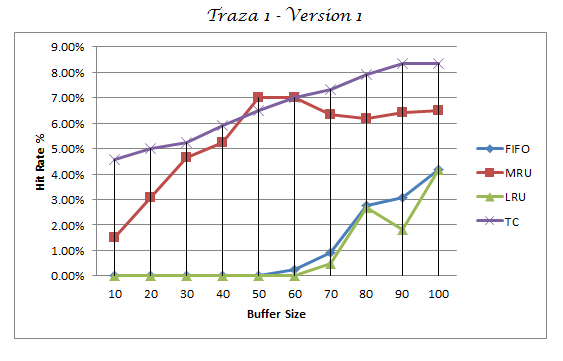
\includegraphics[height=11cm]{img/T1V1.png}
\end{center}  
\begin{center}
  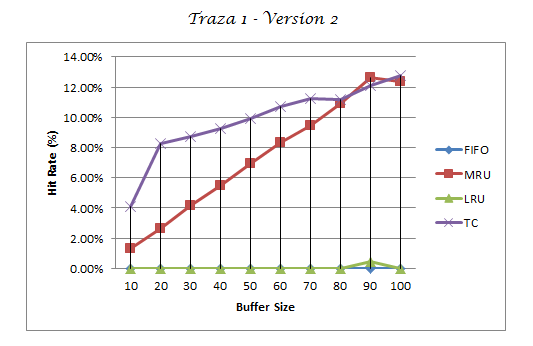
\includegraphics[height=11cm]{img/T1V2.png}
\end{center}  
\begin{center}  
  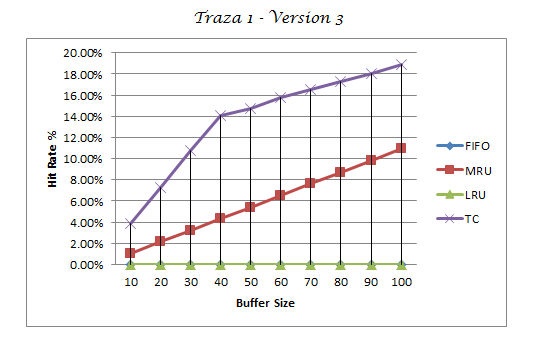
\includegraphics[height=11cm]{img/T1V3.png}
\end{center}  

\subsubsection*{Traza ``2''}
En esta traza lo que hacemos es generar un file scan sobre una tabla cualquiera, en la que se generan 1000 registros. Luego de esto se realiza una carga de registros de una tabla A, luego ocurre lo mismo con una tabla B en la que se reemplazaran en el buffer acordemente segun su tama\~no, finalmente hace una lectura de los registros de A, para luego hacer nuevamente una lectura sobre los registros de B. En la version 1, trabajamos con una cantidad de 50 registros al momento de cargar el buffer, en la 2 con una cantidad de 100 y en la 3 con una cantidad de 200. La escala Buffer Size representa el tama\'no del buffer
\begin{center}
  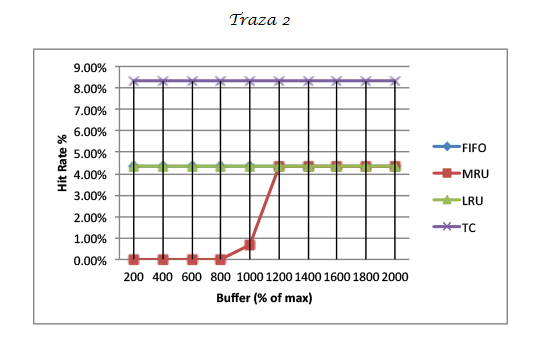
\includegraphics[height=11cm]{img/T2.png}
\end{center}  
\begin{center}
  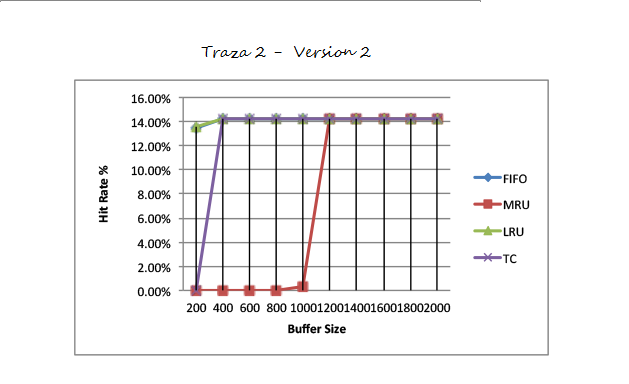
\includegraphics[height=11cm]{img/T2V2.png}
\end{center}  
\begin{center}
  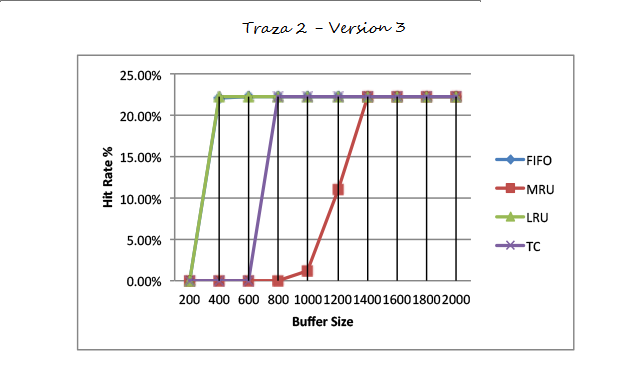
\includegraphics[height=11cm]{img/T2V3.png}
\end{center}  

\subsubsection*{Traza ``Block Nested Loops Join''}
En esta traza se hace un Block Nested Loops Join sobre dos tablas, se carga una tabla de a bloques y la segunda se carga despues de la carga de cada bloque de la primera, esto da la posibilidad de hits sobre los elementos de la segunda tabla. En la version 1, trabajamos con la versi\'on provista por la c\'atedra de SalesXProduct 250, la versi\'on 2 utiliza SalesXProduct 100. La escala Buffer Size representa el tama\'no del buffer
\begin{center}
  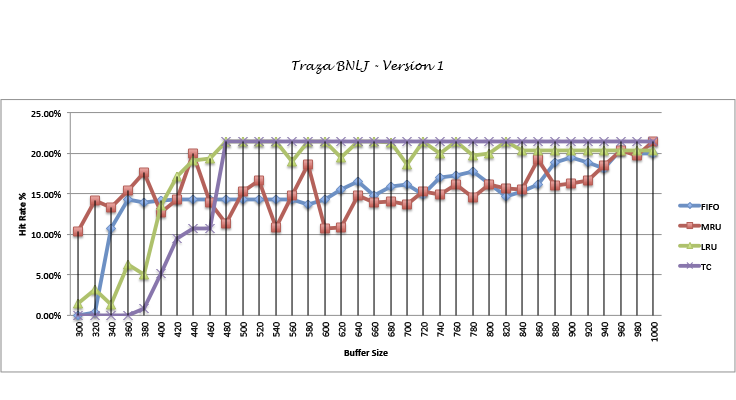
\includegraphics[scale=0.6]{img/T3V1.png}
\end{center}  
\begin{center}
  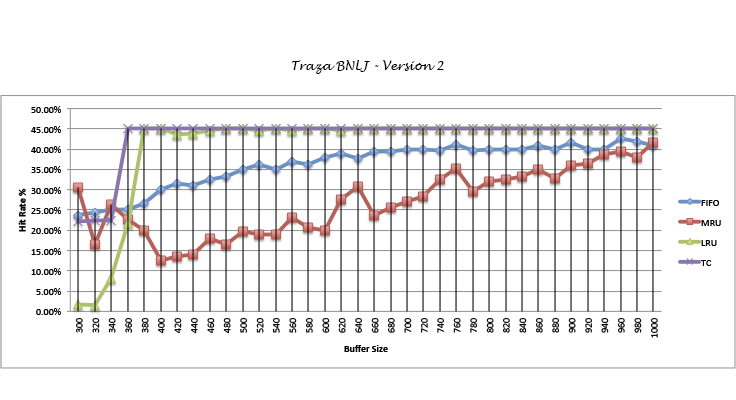
\includegraphics[scale=0.6]{img/T3V2.png}
\end{center}  


\subsection{An\'alisis de los resultados y conclusiones}

De estos resultados se observa un gran contraste entre las estrategias MRU y LRU. La traza 1 contiene un file scan en el medio de la misma, esto es muy malo para LRU y FIFO, puesto que descarta p\'aginas que luego van a volver a ser accedidas por otras que no lo ser\'an; por el contrario, es muy bueno para MRU, que simplemente descarta cada p\'agina apenas se almacena en memoria. Podemos ver que Touch Count se comporta incluso mejor que MRU en esta situaci\'on, las p\'aginas a las que se va a acceder varias veces se cargan en buffer al inicio de la ejecuci\'on, y la segunda lectura hace que pasen a la regi\'on caliente, por lo tanto, el file scan no las va a desalojar, dado que las p\'aginas del file scan entran en la regi\'on fr\'ia y son desalojadas de la misma. Por lo tanto, cuando se vuelve a acceder a las p\'aginas originales, \'estas siguen en la regi\'on caliente y por lo tanto dan hits.

Para la traza 2, el file scan se hace al principio de la ejecuci\'on; esto b\'asicamente vuelve completamente in\'util a la estrategia MRU, puesto que el buffer va a contener a todas las p\'aginas del file scan que entren durante toda la ejecuci\'on (es por esto que reci\'en se ve una cantidad de hits distinta de 0 cuando el buffer es m\'as grande que la cantidad de p\'aginas en la tabla sobre la que se hace file scan). Por el contrario, estrategias como FIFO y LRU no se ven afectadas, ya que simplemente las descartan r\'apidamente al llenarse el buffer. El comportamiento de Touch Count es interesante. Puesto que originalmente el buffer pool est\'a vac\'io, inevitablemente algunas de las p\'aginas del file scan van a quedar en la regi\'on caliente, a\'un sin haber recibido hits, y de ah\'i va a ser muy dif\'icil desalojarlas. Esto redunda en que el buffer efectivo es la mitad de tama\~no, por lo menos hasta que se produzcan hits que muevan dichas p\'aginas a la regi\'on caliente y por ende desalojen esas p\'aginas.

Para las trazas BNLJ, se observan resultados dispares, MRU tiene un funcionamiento que no var\'ia demasiado respecto del tama\'no del buffer, mientras que TC y LRU son en comparaci\'on peores con un buffer peque\'no, pero mucho mejores mientras m\'as grande es el buffer, en particular en la segunda versi\'on de la traza, LRU y TC alcanzan el pico r\'apidamente al crecer el buffer.

\subsection{Tabla de comparaciones}
En funci\'on de los an\'alisis anteriores se presenta la siguiente tabla comparativa de eficiencia de las distintas estrategias en los distintos contextos:
\begin{center}
\scalebox{0.7}{
  %\begin{tabular}{ | l | p{1.6cm} | p{1.6cm} | p{1.6cm} | p{1.6cm} | p{1.6cm} | p{1.6cm} |}
\begin{tabular}{ | l | c | c| c | c | c | c |}
    \hline
    \multirow{2}{*}{Algoritmo} & \multicolumn{2}{c|}{\textbf{Traza 1}} & \multicolumn{2}{c|}{\textbf{Traza 2}} & \multicolumn{2}{c|}{\textbf{BNLJ}} \\
    & Buffer Peque\~no & Buffer grande & Buffer Peque\~no & Buffer grande & Buffer Peque\~no & Buffer grande \\ \hline
    \textbf{Mejor Estrategia/s} & TC & TC & TC/LRU & TC & MRU & TC/LRU \\ \hline
    \textbf{Peor Estrategia/s} & LRU/FIFO & LRU/FIFO & MRU & --- & LRU & MRU \\ \hline
  \end{tabular}}
\end{center}

\\

Se puede ver que el algoritmo Touch Count casi siempre aparece como la mejor o una de las mejores estrategias para las diferentes trazas, existen condiciones en la que no es ideal, esto se debe a que al estar vac\'io y cargar p\'aginas \'estas pueden entrar en la regi\'on caliente sin haber recibido nunca hits, y por definici\'on misma del algoritmo es dif\'icil desalojar las p\'aginas de la regi\'on caliente, por lo tanto se desperdicia espacio del buffer en mantener p\'aginas que no van a dar hits. Esto podr\'ia ser remediado con un proceso que limpie cada la un per\'iodo de tiempo la regi\'on caliente, o por ejemplo que no haya regi\'on caliente hasta que no se produzca un hit, e ir extendiendo la regi\'on caliente hasta alcanzar la mitad a medida que se alcance la cantidad de buffers con hits.

Por otra parte, los algoritmos m\'as simples proporcionan una cantidad de hits a veces considerable, su problema es que todos tienen un caso particular en el que son muy malos, y eso en una base de datos en la que no se sabe con lo que se va a encontrar puede ser muy perjudicial y afectar el rendimiento al provocar muchos miss y sus consiguientes llamados a disco. Por el contrario, Touch Count es mucho m\'as dif\'icil encontrar un caso especial en el que se comporte mucho peor que los otros.

 




 \begin{thebibliography}{2}

\bibitem{ABA} Shallahamer, Craig A. - All about Oracle's Touch Count Algorithm

\bibitem{PPT}http://ebookbrowse.com/187-oracle-touch-count-algorithm-pps-d143194502 
 
\end{thebibliography}


\label{fin}
\end{document}
